\documentclass[sigconf]{acmart}

\usepackage{hyperref}

\usepackage{endfloat}
\renewcommand{\efloatseparator}{\mbox{}} % no new page between figures

\usepackage{booktabs} % For formal tables

\settopmatter{printacmref=false} % Removes citation information below abstract
\renewcommand\footnotetextcopyrightpermission[1]{} % removes footnote with conference information in first column
\pagestyle{plain} % removes running headers

\begin{document}
\title{SIG Proceedings Paper in LaTeX Format}


\author{Jeramy Townsley}
\orcid{1234-5678-9012}
\affiliation{%
  \institution{Institute for Clarity in Documentation}
  \streetaddress{P.O. Box 1212}
  \city{Dublin} 
  \state{Ohio} 
  \postcode{43017-6221}
}
\email{trovato@corporation.com}


% The default list of authors is too long for headers}
\renewcommand{\shortauthors}{B. Trovato et al.}


\begin{abstract}
This paper provides a sample of a \LaTeX\ document which conforms,
somewhat loosely, to the formatting guidelines for
ACM SIG Proceedings.
\end{abstract}

\keywords{ACM proceedings, \LaTeX, text tagging}


\maketitle

\section{Introduction}

Sociological Applications of Big Data

The social sciences have only recently begun to incorporate big data into their analytic frames.  While it may seem that sociology would be a prime fit for big data given the scope of their discipline—describing and theorizing all of society—there have been relatively few thorough explorations of how to apply big data to sociological analysis, particularly in the top sociology journals.  Despite this, outlets have appeared that have taken a lead role in publishing the overlap in these two fields, and solid work has begun. 

This paper will look at four issues.  First, how rapidly have social scientists been incorporating big data into their research and publishing?  Second, what are sites of overlap between sociology and big data, and how is big data defined in terms of what sociologists study.  Third,  what ethical questions have arisen for sociologists about the usage of big data, and how are these issues being addressed?  Fourth, what tools do sociologists have for studying big data?  In the process of looking at these questions, applications of big data by sociologists will be described.

The use of big data to do social science analysis is relatively new.  Using the Google Scholar index to track specific terms by year creates a picture of the rapidity with which social scientists seem to be exploring big data.  Prior to and inclusive of 2005, Google Scholar had 7,560 records containing the phrase, {\em big data} (excluding patents and citations; retrieved 10/5/2017).  Figure 1 shows the cumulative number of records in Google Scholar from 2005-2016 that contain the phrase “big data” plus either “sociology” or “social science.”  There were only 559 in 2005, a mere 7.4\% of the total “big data” references up to that point.  The tipping point seems to be around 2012-2013 when these terms start to appear together.  While after 2015 the number seems to level off, that may simply be an artefact of Google Scholar not yet picking up references since then.  Regardless, there has clearly been a dramatic surge in the last five years.  It is unlikely that all of these represent primary research by social scientists using big data, but it does represent a significant increase in the terms being found in the same articles, implying intersections of interest between the fields.    

Academics publishing in the top sociology journals seem not to be using big data techniques with significant regularity.  The ISI Web of Science tracks impact factors for peer-reviewed journals, and those values can be used to create a general (if not somewhat controversial) list of the top journals in any given field.  Based on the impact factors for 2015, the top ten journals in sociology have a total of 92 usages of the term “big data,” according to a Google Scholar search (10/5/2017).  This is a total search of any timeframe, and as above, not all of these references represent primary research using big data, but simply refer to the term.   The top three journals each have 17 usages of the term, the most of these top ten, while Social Problems contains only 1 reference.  Figure 2 shows these top ten journals along with a count of the usage of the term “big data” from the Google Scholar search.  

In contrast, a relatively new journal began publishing in mid-2014 by Sage, Big Data and Society (BDS).  It self-describes as publishing “ interdisciplinary work principally in the social sciences, humanities and computing and their intersections with the arts and natural sciences about the implications of Big Data for societies.”  While primary research using big data in traditional sociology journals is relatively sparse, BDS publishes twice a year, containing primary research, and other relevant discussions, such as ethics and research methods.  Because of its specificity, it was an important resource for this paper.

Big data has famously been described has having velocity, variety and volume \cite{kitchin14}.  Kitchin (2014) includes five additional concepts: exhaustive in scope, fine-grained resolution, relational, extensional (ability to add fields), and scalable (the latter two concepts sometimes combined under the single concept of flexibility).  In this analysis, Kitchin argues that big can be differentiated from small data specifically along these eight axes, and that while some small datasets may have characteristics of big data, such as strong relationality or wide variety, there is little overlap along the other axes.  In their 2016 review, Kitchin and McArdle test 26 datasets that have previously been defined as big data for their ‘fit’ based on these differentiating concepts.  They conclude that not only do not all datasets fit all of the criteria Kitchin described, but they also do not all fit the original descriptions of volume, velocity and variety.  However, they do believe that all of the 26 datasets are characterized by velocity and exhaustivity, which they describe concisely as, “real time flow of data across a whole system” that produces a large dataset.  The other descriptive concepts are still relevant, and may be pertinent to some big datasets, but not to others.

This is an example on how to refer to Figure \ref{f:figure1}

\begin{figure}
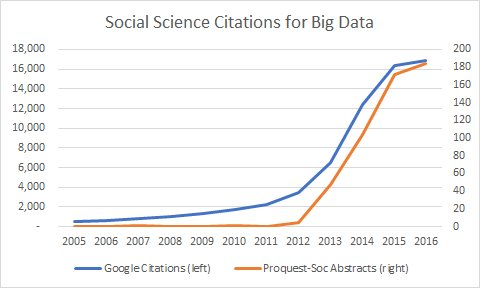
\includegraphics[width=\columnwidth]{images/figure1}
\caption{A sample black and white graphic
that has been resized with the \texttt{includegraphics} command.}
\label{f:figure1}
\end{figure}




\begin{acks}

  temp

\end{acks}

\bibliographystyle{ACM-Reference-Format}
\bibliography{report} 

\end{document}
